\documentclass[a4paper,12pt]{article}
\usepackage[utf8]{inputenc}
\usepackage[T1]{fontenc}
\usepackage{lmodern}
\usepackage{geometry}
\usepackage{setspace}
\usepackage{fancyhdr}
\usepackage{hyperref}
\usepackage{amsmath}
\usepackage{amsfonts}
\usepackage{amssymb}
\usepackage{mathtools}
\usepackage{float}
\usepackage{tabularx}
\usepackage{enumitem}
\usepackage{graphicx}
\usepackage{ragged2e}
\usepackage[spanish]{babel}
\usepackage{booktabs}
\usepackage{longtable}
\usepackage{multirow}
\usepackage{xcolor}
\usepackage{microtype}
\usepackage{caption}
\usepackage{textcomp}
\newcommand{\euro}{\texteuro}
\newcommand{\E}{\mathbb{E}}
\newcommand{\Var}{\mathrm{Var}}
\newcommand{\Cov}{\mathrm{Cov}}
\newcommand{\VaR}{\mathrm{VaR}}
\newcommand{\TVaR}{\mathrm{TVaR}}
\addto\captionsspanish{\renewcommand{\tablename}{Tabla}}
\addto\captionsspanish{\renewcommand{\figurename}{Figura}}
\captionsetup{font=small,labelfont=bf}

% Configuración de márgenes
\geometry{left=2.5cm,right=2.5cm,top=3cm,bottom=3cm}

% Configuración de encabezados y pies de página
\pagestyle{fancy}
\fancyhf{}
\renewcommand{\headrulewidth}{0pt}
\fancyfoot[C]{\thepage}

% Configuración de interlineado
\onehalfspacing
\justifying

% Configuración de hipervínculos
\hypersetup{
    hidelinks,
    colorlinks=false
}

\begin{document}

% Primera página (Título, Resumen y Abstract)
\begin{titlepage}
    \centering
    \vspace*{0.1cm}
    \huge\textbf{Tema 1: Preguntas de repaso}\\
    \vspace{1cm}
    \small{Luiz Alberto Luzuriaga Izquierdo}\\
    \vspace{0.1cm}
    Facultad de ciencias económicas, empresariales y turismo. \\
    \vspace{0.1cm}
    Universidad de Alcalá de Henares. \\
    \vspace{0.1cm}
    Curso 2026-2027\\
    \vspace{0.5cm}

{\bfseries Resumen}

\vspace{0.1cm}
\noindent
\begin{justify}
Respuestas razonadas a las tres preguntas de repaso del tema. Tema 1 (Teoría de la utilidad y decisiones bajo riesgo): Funciones de utilidad CRRA y CARA, coeficiente de Arrow-Pratt, equivalente cierto, prima de riesgo y zona de acuerdo cedente-reasegurador.\\\\
\vspace{0.1cm}
\noindent
\textbf{Palabras clave}: utilidad esperada, aversión al riesgo, reaseguro, preguntas de repaso.
\end{justify}
\begin{center}
    {\bfseries Abstract}
\end{center}
\vspace{0.1cm}
\noindent
\begin{justify}
Class work for Topic 1 of Actuarial Mathematics of Stability and Solvency of Insurance Activity: review questions with actuarial reasoning and numerical evidence.\\\\
\vspace{0.1cm}
\noindent
\textbf{Keywords}: expected utility, risk aversion, reinsurance, review questions.
\end{justify}

\end{titlepage}

% Índice
\newpage\pagenumbering{gobble}
\renewcommand{\contentsname}{Índice}
\newgeometry{left=4cm, right=4cm, top=3cm, bottom=2.5cm}
\tableofcontents

\restoregeometry
\newpage
\numberwithin{equation}{section}
\pagenumbering{arabic}
\setcounter{page}{1}

\section{Tema 1: Teoría de la utilidad y decisiones bajo riesgo}
\label{sec:tema1repaso}
\noindent
Respuestas razonadas a las tres preguntas de repaso del tema. Material de referencia: diapositivas del Tema 1 (Prof. Hugo González Riera).

\subsection{Pregunta 1 -- El l\'imite $\gamma\to1$ de la utilidad CRRA es la logar\'itmica}

\noindent\textbf{Enunciado.} Demuestra que el caso l\'imite $\gamma\to1$ de la utilidad potencia (CRRA) es la utilidad logar\'itmica $u(w)=\log w$.

\subsubsection*{Planteamiento: hay un detalle que hay que tratar con cuidado}
La familia CRRA se escribe $u_\gamma(w)=\dfrac{w^{1-\gamma}}{1-\gamma}$, con $w>0$ y $\gamma\neq1$. Si se toma el l\'imite de esa expresi\'on \emph{tal cual}, no existe: cuando $\gamma\to1$ el numerador tiende a $w^0=1$ y el denominador a $0$, de modo que $u_\gamma(w)\to\pm\infty$ seg\'un el lado por el que nos acerquemos a $1$. Esto no es un problema real, porque la utilidad de von Neumann--Morgenstern est\'a definida \emph{salvo transformaci\'on af\'in positiva}: $u$ y $a\,u+b$ con $a>0$ producen exactamente las mismas decisiones. El l\'imite correcto es, por tanto, el de la versi\'on normalizada
\begin{equation}\label{eq:norm}
\tilde u_\gamma(w)=u_\gamma(w)-\frac{1}{1-\gamma}=\frac{w^{1-\gamma}-1}{1-\gamma},
\end{equation}
que se obtiene restando la constante $b=-1/(1-\gamma)$ (y $a=1$), con lo que $\tilde u_\gamma(1)=0$.

\subsubsection*{Demostraci\'on}
Fijemos $w>0$. Escribimos $w^{1-\gamma}=e^{(1-\gamma)\ln w}$ y llamamos $\varepsilon=1-\gamma\to0$. Entonces
\[
\tilde u_\gamma(w)=\frac{e^{\varepsilon\ln w}-1}{\varepsilon}.
\]
Es una indeterminaci\'on $0/0$. Aplicando la regla de L'H\^opital respecto de $\varepsilon$ (o, directamente, reconociendo la derivada de $\varepsilon\mapsto e^{\varepsilon\ln w}$ en $\varepsilon=0$):
\[
\lim_{\varepsilon\to0}\frac{e^{\varepsilon\ln w}-1}{\varepsilon}=\lim_{\varepsilon\to0}\frac{(\ln w)\,e^{\varepsilon\ln w}}{1}=\ln w .
\]
Por tanto $\tilde u_\gamma(w)\to\ln w$ cuando $\gamma\to1$, y la convergencia es uniforme sobre compactos de $(0,\infty)$ (basta el desarrollo $e^{x}=1+x+O(x^2)$).

\subsubsection*{Comprobaciones de coherencia (lo que la prueba debe preservar)}
\begin{enumerate}[leftmargin=*]
\item \textbf{Aversi\'on relativa.} Para $\tilde u_\gamma$: $\tilde u_\gamma'(w)=w^{-\gamma}$, $\tilde u_\gamma''(w)=-\gamma w^{-\gamma-1}$, luego $\rho(w)=-w\,\tilde u''/\tilde u'=\gamma$. Para $\ln w$: $u'=1/w$, $u''=-1/w^2$ y $\rho(w)=1$. El l\'imite conserva el coeficiente: $\rho=\gamma\to1$.
\item \textbf{Equivalente cierto.} Para una riqueza aleatoria $\widetilde W>0$ y $\gamma\neq1$, de $u_\gamma(CE)=\E[u_\gamma(\widetilde W)]$ resulta
\[CE_\gamma=\Big(\E\big[\widetilde W^{\,1-\gamma}\big]\Big)^{\frac1{1-\gamma}}.\]
Cuando $\gamma\to1$ es una forma $1^\infty$: $\ln CE_\gamma=\dfrac{\ln \E[\widetilde W^{\varepsilon}]}{\varepsilon}\to\dfrac{\E[\ln\widetilde W]\,\varepsilon}{\varepsilon}=\E[\ln\widetilde W]$, es decir
\[CE_1=\exp\big(\E[\ln\widetilde W]\big),\]
la \emph{media geom\'etrica} de la riqueza final. Este es un resultado \'util: con utilidad logar\'itmica el decisor valora una lotería por su media geom\'etrica, que siempre es $\le$ la media aritm\'etica (Jensen).
\item \textbf{Orden de preferencias.} Como $\tilde u_\gamma\to\ln$ y la esperanza es continua en el l\'imite, el orden de preferencias entre cualesquiera dos loter\'ias converge al orden logar\'itmico: la familia es continua en $\gamma$.
\end{enumerate}

\subsubsection*{Comprobaci\'on num\'erica con el Caso 2 de la sesi\'on}
Con $w=10.000$ y $X=+2.000$ o $-1.500$ con probabilidad $1/2$, el CE para $\gamma=1$ es $\sqrt{12.000\cdot8.500}=10.099{,}5$ (media geom\'etrica); para $\gamma=0{,}99$ y $\gamma=1{,}01$ la f\'ormula general da $10.101{,}0$ y $10.098{,}0$ respectivamente, a ambos lados del valor l\'imite y con el sentido esperado (el CE decrece con $\gamma$).

\paragraph{Conclusi\'on.} La utilidad logar\'itmica de Bernoulli no es una familia aparte: es el miembro $\gamma=1$ de la CRRA, y se recupera como l\'imite de la forma normalizada \eqref{eq:norm}. La utilidad no depende de la constante aditiva, por lo que ``el l\'imite de $w^{1-\gamma}/(1-\gamma)$'' debe entenderse siempre salvo transformaci\'on af\'in.

\bigskip\hrule\bigskip

\subsection{Pregunta 2 -- Por qu\'e la prima exponencial no depende de la riqueza y la potencia s\'i}

\noindent\textbf{Enunciado.} Para una utilidad exponencial de par\'ametro $\alpha$, explica por qu\'e la prima $P=\frac1\alpha\ln M_X(\alpha)$ no depende de la riqueza $w$, mientras que para una potencia (CRRA) s\'i depende. ?`Qu\'e implicaci\'on pr\'actica tiene al elegir un modelo para pricing de reaseguro?

\subsubsection*{La prima m\'axima se define por indiferencia}
El decisor con riqueza $w$ y utilidad $u$ paga como m\'aximo la cantidad $P$ que le deja indiferente entre transferir el riesgo $X$ y retenerlo:
\begin{equation}\label{eq:equil}
u(w-P)=\E\big[u(w-X)\big].
\end{equation}

\paragraph{Caso CARA, $u(w)=-e^{-\alpha w}/\alpha$.} El lado izquierdo es $-\frac1\alpha e^{-\alpha w}e^{\alpha P}$. El derecho es $-\frac1\alpha\,\E\big[e^{-\alpha(w-X)}\big]=-\frac1\alpha e^{-\alpha w}\,\E\big[e^{\alpha X}\big]$. El factor $e^{-\alpha w}$ \emph{aparece multiplicando a ambos lados} y se cancela:
\[
e^{\alpha P}=M_X(\alpha)\;\Longrightarrow\;P=\frac1\alpha\ln M_X(\alpha)=\frac{K_X(\alpha)}{\alpha},
\]
con $K_X=\ln M_X$ la funci\'on generadora de cumulantes. La causa de fondo es que la exponencial convierte \emph{sumas} de riqueza en \emph{productos}: $u(w-x)=e^{-\alpha w}\cdot u(-x)$. Es la \'unica familia (salvo af\'in) con aversi\'on absoluta constante, $r(w)=\alpha$.

\paragraph{Caso CRRA, $u(w)=w^{1-\gamma}/(1-\gamma)$.} Ahora no hay factorizaci\'on posible: $(w-x)^{1-\gamma}$ no separa $w$ de $x$. La ecuaci\'on \eqref{eq:equil} da
\[
(w-P)^{1-\gamma}=\E\big[(w-X)^{1-\gamma}\big]\;\Longrightarrow\;P(w)=w-\Big(\E\big[(w-X)^{1-\gamma}\big]\Big)^{\frac1{1-\gamma}},
\]
que depende de $w$ de forma esencial. Intuitivamente, $\rho(w)=\gamma$ constante implica que la aversi\'on \emph{absoluta} $r(w)=\gamma/w$ decrece con la riqueza: el mismo riesgo pesa menos a quien tiene m\'as capital.

\subsubsection*{Ejemplo num\'erico}
Sea $X=5.000$ con probabilidad $0{,}2$ y $0$ en otro caso ($\E[X]=1.000$). Con $\alpha=2\cdot10^{-4}$: $P=\frac{1}{\alpha}\ln(0{,}8+0{,}2\,e^{1})=1.477{,}0$ para \emph{cualquier} $w$. Con CRRA $\gamma=2$ (donde $P(w)=w-\big(0{,}8/w+0{,}2/(w-5.000)\big)^{-1}$):
\begin{center}
\begin{tabular}{r r r}
\toprule
Riqueza $w$ & $P$ CARA & $P$ CRRA ($\gamma=2$)\\
\midrule
6.000 & 1.477,0 & 3.000,0\\
10.000 & 1.477,0 & 1.666,7\\
20.000 & 1.477,0 & 1.250,0\\
50.000 & 1.477,0 & 1.087,0\\
200.000 & 1.477,0 & 1.020,4\\
\bottomrule
\end{tabular}
\end{center}
\begin{figure}[H]\centering
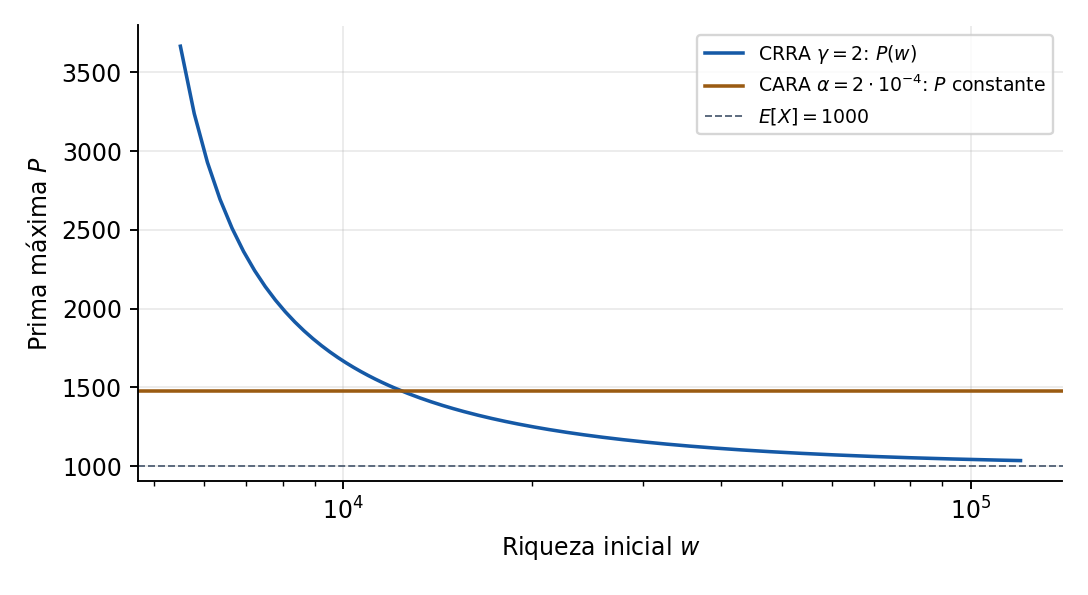
\includegraphics[width=.72\linewidth]{t1_f_repaso2.png}
\caption{La prima CARA es constante; la CRRA decrece hacia $\E[X]$ al crecer $w$ (y explota cuando $w\downarrow5.000$, donde la ruina es posible).}
\end{figure}
Dos lecturas: (i) un decisor CRRA con riqueza cercana a la p\'erdida m\'axima pagar\'a una prima enorme (con $w\le5.000$ la utilidad esperada es $-\infty$ y el riesgo es inasegurable para \'el), mientras que con mucha riqueza la prima se acerca a la pura; (ii) CARA ``no reconoce'' que un decisor m\'as capitalizado deber\'ia ser menos averso, de ah\'i que $\alpha$ no se calibre una vez para siempre.

\subsubsection*{Implicaci\'on para el pricing de reaseguro}
\begin{itemize}[leftmargin=*]
\item \textbf{Observabilidad.} En reaseguro la riqueza efectiva del cedente (y a veces la del propio reasegurador) es informaci\'on privada, cambiante y dif\'icil de definir (capital econ\'omico, SCR, fondos propios admisibles). La prima exponencial exige solo la distribuci\'on del riesgo y un \'unico par\'ametro $\alpha$: es \emph{trasladable} entre cedentes y fechas.
\item \textbf{Aditividad.} Para riesgos independientes, $M_{X+Y}=M_XM_Y$ y por tanto $P(X+Y)=P(X)+P(Y)$: la prima de una cartera es la suma de las primas de sus partes, algo muy conveniente para contratos por tramos o por cuentas. La prima CRRA no es aditiva.
\item \textbf{Consistencia en capas.} La prima exponencial es \emph{iterativa}: $P(X)=P\big(P(X\mid Y)\big)$, de modo que fijar el precio en dos pasos (primero condicionando a un evento y luego agregando) da el mismo resultado que fijarlo de golpe. Evita incoherencias entre tratados superpuestos.
\item \textbf{Contrapartida.} Con CARA no hay efecto riqueza: un gran reasegurador no ``abarata'' sus primas por tener m\'as capital, salvo que se recalibre $\alpha$ (por ejemplo $\alpha\approx1/\text{(tolerancia al riesgo)}$); y $M_X(\alpha)=\infty$ si las colas son pesadas, de modo que la prima exponencial no existe para riesgos tipo Pareto. Para ellos se usan otros principios (varianza, desviaci\'on est\'andar, distorsi\'on de Wang) o una calibraci\'on basada en medidas de cola como el TVaR.
\end{itemize}
CRRA queda para decisiones donde el riesgo escala con el balance: asignaci\'on de activos, capital en \% de los fondos propios, apetito de riesgo de una gestora. En resumen: \textbf{CARA para primas de reaseguro, CRRA para inversi\'on}.

\bigskip\hrule\bigskip

\subsection{Pregunta 3 -- La zona de acuerdo es no vac\'ia si $\alpha_R<\alpha_C$}

\noindent\textbf{Enunciado.} Un cedente tiene aversi\'on absoluta $\alpha_C$ y un reasegurador $\alpha_R<\alpha_C$. Razona, sin hacer c\'alculos, por qu\'e la zona de acuerdo $[P^-,P^+]$ es no vac\'ia y qu\'e ocurre con su anchura si $\alpha_R\to0$.

\subsubsection*{Razonamiento}
Con utilidades exponenciales, las dos primas del puente hacia el reaseguro son (ambas independientes de la riqueza):
\[
P^+=\frac{K_X(\alpha_C)}{\alpha_C},\qquad P^-=\frac{K_X(\alpha_R)}{\alpha_R},\qquad K_X=\ln M_X .
\]
Ambas son la misma funci\'on $\Pi(\alpha)=K_X(\alpha)/\alpha$ evaluada en la aversi\'on de cada parte. Basta, entonces, ver que \textbf{$\Pi$ es creciente en $\alpha$}.

\paragraph{$\Pi$ es creciente.} $K_X$ es convexa (es el logaritmo de una funci\'on generadora de momentos, y por Hölder $\ln M$ es convexa) y $K_X(0)=0$. Para $0<a<b$ se tiene $a=\tfrac ab\,b+(1-\tfrac ab)\,0$, de modo que por convexidad
\[
K_X(a)\le\frac ab K_X(b)+\Big(1-\frac ab\Big)K_X(0)=\frac ab K_X(b)\;\Longrightarrow\;\frac{K_X(a)}{a}\le\frac{K_X(b)}{b}.
\]
Geom\'etricamente, $\Pi(\alpha)$ es la pendiente de la cuerda que une el origen con $(\alpha,K_X(\alpha))$, y esa pendiente crece con $\alpha$ para una curva convexa que parte del origen. La desigualdad es estricta salvo que $K_X$ sea lineal, es decir, salvo que $X$ sea constante (riesgo degenerado).

\paragraph{Consecuencia.} Si $\alpha_R<\alpha_C$ entonces $P^-=\Pi(\alpha_R)<\Pi(\alpha_C)=P^+$: la zona de acuerdo es no vac\'ia para cualquier riesgo no degenerado. Si $\alpha_R=\alpha_C$ colapsa a un punto (no hay ganancia de intercambio). La condici\'on de existencia es independiente de la riqueza de las partes. Nota de borde: si $\alpha_C$ supera la abscisa de convergencia de $M_X$ (para la Gamma, $1/\theta$), $P^+=\infty$ y el cedente aceptar\'ia cualquier precio; no es un resultado razonable en la pr\'actica, solo avisa de que el modelo exponencial se rompe.

\paragraph{L\'imite $\alpha_R\to0$.} Como $K_X(0)=0$ y $K_X'(0)=\E[X]$, por definici\'on de derivada
\[
\lim_{\alpha_R\to0}P^-=\lim_{\alpha_R\to0}\frac{K_X(\alpha_R)-K_X(0)}{\alpha_R}=\E[X].
\]
Un reasegurador neutral al riesgo cobra la prima pura y la zona se ensancha hasta su m\'aximo, $[\E[X],P^+]$, de anchura $P^+-\E[X]$ (todo el recargo que el cedente est\'a dispuesto a pagar). Para riesgos peque\~nos, $\Pi(\alpha)\approx\E[X]+\tfrac12\alpha\Var[X]$, as\'i que la anchura es $\approx\tfrac12(\alpha_C-\alpha_R)\Var[X]$: es lineal en la diferencia de aversiones.

\subsubsection*{Verificaci\'on con el Caso 1 (solo como comprobaci\'on)}
Para $X=\theta Y$, $Y\sim\Gamma(2,1)$, $\theta=500$: $K_X(\alpha)=-2\ln(1-500\alpha)$. Con $\alpha_C=6\cdot10^{-4}$ y $\alpha_R=3\cdot10^{-4}$ se obtiene $P^+=1.188{,}9$, $P^-=1.083{,}5$ y anchura $105{,}5$; el l\'imite $\alpha_R\to0$ da $P^-\to1.000$ y anchura $188{,}9$ (el $18{,}9\%$ de $\E[X]$). La aproximaci\'on de segundo orden dar\'ia $\tfrac12(3\cdot10^{-4})(500.000)=75$, menor que el valor exacto $105{,}5$ porque el riesgo es asim\'etrico y la convexidad de $K_X$ aporta el resto.
\begin{figure}[H]\centering
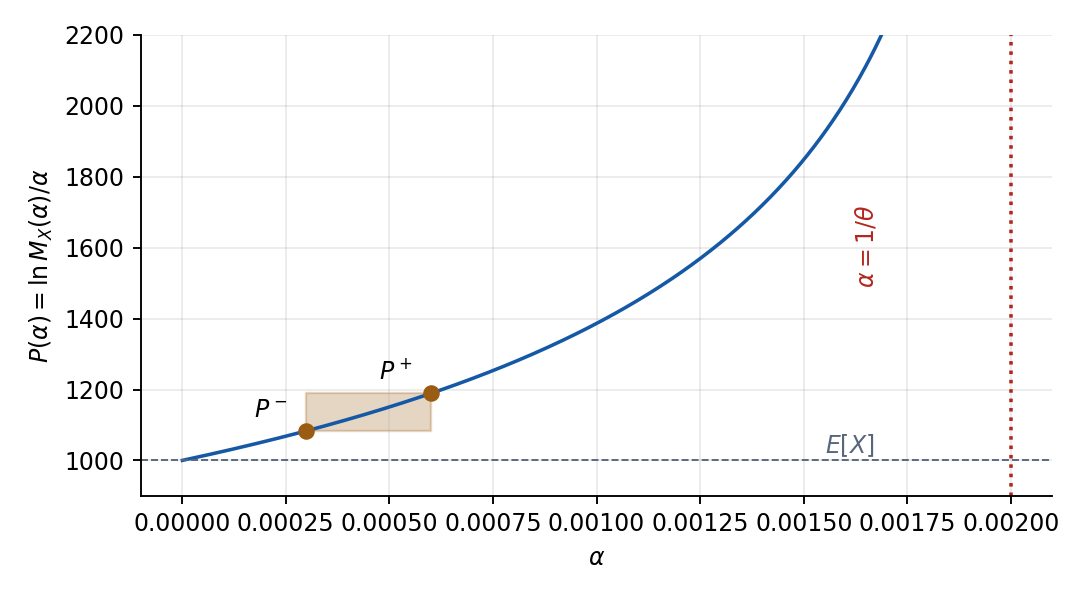
\includegraphics[width=.72\linewidth]{t1_f_repaso3.png}
\caption{$\Pi(\alpha)=K_X(\alpha)/\alpha$ crece con $\alpha$ y parte de $\E[X]$; el \'area sombreada es la zona de acuerdo del Caso 1.}
\end{figure}

\paragraph{Una observaci\'on de segundo nivel.} Que exista margen no significa que el contrato \'optimo sea ceder el 100\,\%. Con utilidades exponenciales, el reparto Pareto-eficiente de un riesgo es proporcional a las tolerancias $\tau_i=1/\alpha_i$ (Borch, 1962): el reasegurador del Caso 1 asumir\'ia $\tau_R/(\tau_R+\tau_C)=2/3$ del riesgo y el cedente retendr\'ia $1/3$. La cesi\'on total es solo el caso en que el reasegurador es neutral.

\subsubsection*{Referencias}
\begin{itemize}[leftmargin=*,itemsep=0pt]
\item Kaas, R., Goovaerts, M., Dhaene, J. y Denuit, M. (2008). \emph{Modern Actuarial Risk Theory} (2.\textordfeminine\ ed.). Springer. Cap.~1.
\item Pratt, J. W. (1964). Risk aversion in the small and in the large. \emph{Econometrica}, 32, 122--136.
\item Arrow, K. J. (1971). \emph{Essays in the Theory of Risk-Bearing}. Markham.
\item Borch, K. (1962). Equilibrium in a reinsurance market. \emph{Econometrica}, 30, 424--444.
\item B\"uhlmann, H. (1970). \emph{Mathematical Methods in Risk Theory}. Springer.
\end{itemize}

\end{document}
